\chapter{HTC Testbed}
\label{app:A}
\section{Location information of the Grid}
\begin{wrapfigure}{r}{5.5cm}
\includegraphics[width=5.5cm]{./pics/angle.png}
\label{fig:height}
\end{wrapfigure}
The coordinates of the vertices are as given in the table \ref{tab:htc34xy}. We use EKMB1101112 PIR sensors from Panasonic, with detection angle of $82^\circ$.
PIR nodes are placed on the ceiling which is at a height of 3m. From this information we can compute the radius of the field of view of the PIR sensors as follows:\\\\
$h=3m, a = 82^{\circ}$\\
$r=h\cdot tan(\frac{a}{2})$\\
$r=2.6m$\\






\begin{table}[]
\centering
\caption{Coordinates of the vertices of the sensor network}
\label{tab:htc34xy}
\begin{tabular}{|c|c|c|}
\hline
vetrex & x   & y   \\ \hline
1      & 0   & 0   \\ \hline
2      & 0   & 2.2 \\ \hline
3      & 2.5 & 0   \\ \hline
4      & 2.5 & 2.2 \\ \hline
5      & 5   & 0   \\ \hline
6      & 5   & 2.2 \\ \hline
7      & 7.5 & 0   \\ \hline
8      & 7.5 & 2.2 \\ \hline
\end{tabular}
\end{table}

\begin{table}[]
\centering
\caption{Euclidean distances between vertices}
\label{tab:dist}
\begin{tabular}{|c|c|c|c|c|c|c|c|c|}
\hline
vertices & 1    & 2    & 3    & 4    & 5    & 6    & 7    & 8    \\ \hline
1        & 0.00 & 2.00 & 2.50 & 3.20 & 5.00 & 5.39 & 7.50 & 7.76 \\ \hline
2        & 2.00 & 0.00 & 3.20 & 2.50 & 5.39 & 5.00 & 7.76 & 7.50 \\ \hline
3        & 2.50 & 3.20 & 0.00 & 2.00 & 2.50 & 3.20 & 5.00 & 5.39 \\ \hline
4        & 3.20 & 2.50 & 2.00 & 0.00 & 3.20 & 2.50 & 5.39 & 5.00 \\ \hline
5        & 5.00 & 5.39 & 2.50 & 3.20 & 0.00 & 2.00 & 2.50 & 3.20 \\ \hline
6        & 5.39 & 5.00 & 3.20 & 2.50 & 2.00 & 0.00 & 3.20 & 2.50 \\ \hline
7        & 7.50 & 7.76 & 5.00 & 5.39 & 2.50 & 3.20 & 0.00 & 2.00 \\ \hline
8        & 7.76 & 7.50 & 5.39 & 5.00 & 3.20 & 2.50 & 2.00 & 0.00 \\ \hline
\end{tabular}
\end{table}

The distances between all the sensor nodes are represented in a matrix form and is as given in the table \ref{tab:dist} . The radius of the PIR sensor is 2.6m thus any 2 sensors located less than 5.2m(2r) apart are considered neighboring sensors. The adjacecy matrix is obtained as shown in the table \ref{tab:am}

\begin{table}[]
\centering
\caption{Adjacency matrix}
\label{tab:am}
\begin{tabular}{|c|c|c|c|c|c|c|c|c|}
\hline
vertices & 1 & 2 & 3 & 4 & 5 & 6 & 7 & 8 \\ \hline
1        & 0 & 1 & 1 & 1 & 1 & 0 & 0 & 0 \\ \hline
2        & 1 & 0 & 1 & 1 & 0 & 1 & 0 & 0 \\ \hline
3        & 1 & 1 & 0 & 1 & 1 & 1 & 1 & 0 \\ \hline
4        & 1 & 1 & 1 & 0 & 1 & 1 & 0 & 1 \\ \hline
5        & 1 & 0 & 1 & 1 & 0 & 1 & 1 & 1 \\ \hline
6        & 0 & 1 & 1 & 1 & 1 & 0 & 1 & 1 \\ \hline
7        & 0 & 0 & 1 & 0 & 1 & 1 & 0 & 1 \\ \hline
8        & 0 & 0 & 0 & 1 & 1 & 1 & 1 & 0 \\ \hline
\end{tabular}
\end{table}

\chapter{Tokyo Testbed}
\label{app:B}

The coordinates of the vertices in Tokyo testbed are not explicitly specified. The information available are the room layout map as shown in figure \ref{fig:casas}, pir sensor field of view given as $1.2m \times 1.2m$ and the average distance between the sensors as 1.2m in \cite{crandall2011tracking}. Assuming that the given layout is to scale and the distance between sensors 27 and 22 as 1.2m, the coordinates of all the sensors are computed. We start by placing the origin(0,0) at vertex 30 and measure the distance of every vertex from the x and y axis which gives the coordinates of all vertices on the grid. The coordinates thus obtained are as shown in the table \ref{tab:wsuxy}. No triggers was found for sensor 38 in the dataset, hence sensor 38 is not considered.


\begin{table}[]
\centering
\caption{Coordinates obtained for the vertices}
\label{tab:wsuxy}
\begin{tabular}{|c|c|c|c|c|c|c|c|c|c|c|c|}
\hline
vertices & x    & y     & vertices & x    & y     & vertices & x     & y     & vertices & x     & y     \\ \hline
1        & 4.40 & 5.60  & 12       & 3.60 & 0.00  & 23       & 1.20  & 2.00  & 34       & -0.60 & 5.00  \\ \hline
2        & 4.40 & 4.00  & 13       & 3.60 & -1.20 & 24       & 1.20  & 0.80  & 36       & -1.40 & 4.40  \\ \hline
3        & 4.40 & 3.20  & 14       & 2.40 & 3.60  & 25       & 1.20  & 0.00  & 37       & -1.80 & 4.80  \\ \hline
4        & 4.80 & 1.20  & 15       & 2.40 & 3.20  & 26       & 1.20  & -1.20 & 39       & -1.40 & -0.20 \\ \hline
5        & 4.80 & 0.00  & 16       & 2.40 & 2.00  & 27       & 0.00  & 3.20  & 40       & -2.20 & 1.88  \\ \hline
6        & 4.80 & -1.20 & 17       & 2.40 & 0.80  & 28       & 0.00  & 2.00  & 41       & -2.20 & 0.68  \\ \hline
7        & 3.40 & 5.60  & 18       & 2.40 & 0.00  & 29       & 0.00  & 0.80  & 42       & -2.20 & -0.52 \\ \hline
8        & 3.40 & 4.40  & 19       & 1.20 & 4.80  & 30       & 0.00  & 0.00  & 43       & -3.40 & 1.88  \\ \hline
9        & 3.40 & 3.20  & 20       & 0.60 & 4.64  & 31       & 0.00  & -1.20 & 44       & -3.40 & 0.68  \\ \hline
10       & 3.90 & 2.00  & 21       & 1.20 & 3.60  & 32       & -1.20 & -0.40 & 45       & -3.40 & -0.52 \\ \hline
11       & 3.60 & 1.20  & 22       & 1.20 & 3.20  & 33       & -0.60 & 3.80  &          &       &       \\ \hline
\end{tabular}
\end{table}




%\begin{figure}
%\centering
%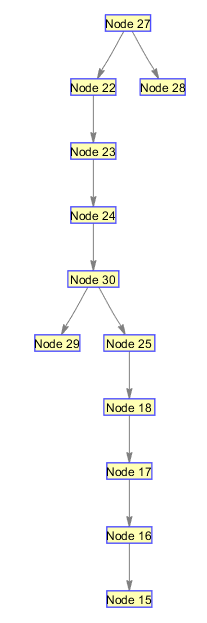
\includegraphics{./pics/MST4x3_1.png}
%\caption{MST for the $4 \times 3$ layout}
%\label{fig:MST4x3}
%\end{figure}
%
%
%\begin{figure}
%\centering
%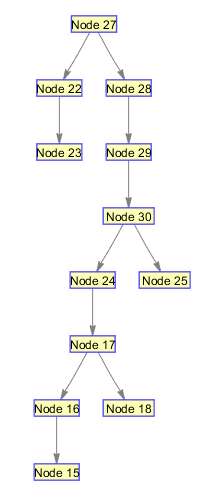
\includegraphics{./pics/MST4x3_2.png}
%\caption{MST for the $4 \times 3$ layout}
%\label{fig:MST4x3_2}
%\end{figure}







